\documentclass[14pt]{beamer}
\usepackage[T2A]{fontenc}
\usepackage[utf8]{inputenc}
\usepackage[english,russian]{babel}
\usepackage{amssymb,amsfonts,amsmath,mathtext}
\usepackage{cite,enumerate,float,indentfirst}

\graphicspath{{../images/}{images/}} 



% \usetheme[secheader]{Boadilla}
% \usecolortheme{seahorse}

\usetheme{Pittsburgh}
\usecolortheme{whale}

\beamertemplatenavigationsymbolsempty

\newcommand{\todo}{\alert}
%%% Основные сведения %%%
\newcommand{\thesisAuthor}             % Диссертация, ФИО автора
{%
    \texorpdfstring{% \texorpdfstring takes two arguments and uses the first for (La)TeX and the second for pdf
        \todo{Фамилия Имя Отчество автора}% так будет отображаться на титульном листе или в тексте, где будет использоваться переменная
    }{%
        Фамилия, Имя Отчество% эта запись для свойств pdf-файла. В таком виде, если pdf будет обработан программами для сбора библиографических сведений, будет правильно представлена фамилия.
    }%
}
\newcommand{\thesisAuthorShort}        % Диссертация, ФИО автора инициалами
{\todo{И.О.~Фамилия}}

\newcommand{\thesisUdk}                % Диссертация, УДК
{\todo{xxx.xxx}}
\newcommand{\thesisTitle}              % Диссертация, название
{\texorpdfstring{\todo{\MakeUppercase{Название диссертационной работы}}}{Название диссертационной работы}}
\newcommand{\thesisSpecialtyNumber}    % Диссертация, специальность, номер
{\texorpdfstring{\todo{XX.XX.XX}}{XX.XX.XX}}
\newcommand{\thesisSpecialtyTitle}     % Диссертация, специальность, название
{\texorpdfstring{\todo{Название специальности}}{Название специальности}}
\newcommand{\thesisDegree}             % Диссертация, ученая степень
{\todo{кандидата физико-математических наук}}
\newcommand{\thesisDegreeShort}        % Диссертация, ученая степень, краткая запись
{\todo{канд. физ.-мат. наук}}
\newcommand{\thesisCity}               % Диссертация, город написания диссертации
{\todo{Город}}
\newcommand{\thesisYear}               % Диссертация, год написания диссертации
{\todo{20XX}}
\newcommand{\thesisOrganization}       % Диссертация, организация
{\todo{Название учреждения, в~котором выполнялась данная диссертационная работа}}
\newcommand{\thesisOrganizationShort}  % Диссертация, краткое название организации для доклада
{\todo{НазУчДисРаб}}

\newcommand{\thesisInOrganization}     % Диссертация, организация в предложном падеже: Работа выполнена в ...
{\todo{учреждении, в~котором выполнялась данная диссертационная работа}}

\newcommand{\supervisorFio}            % Научный руководитель, ФИО
{\todo{Фамилия Имя Отчество}}
\newcommand{\supervisorRegalia}        % Научный руководитель, регалии
{\todo{уч. степень, уч. звание}}
\newcommand{\supervisorFioShort}       % Научный руководитель, ФИО
{\todo{И.О.~Фамилия}}
\newcommand{\supervisorRegaliaShort}   % Научный руководитель, регалии
{\todo{уч.~ст.,~уч.~зв.}}


\newcommand{\opponentOneFio}           % Оппонент 1, ФИО
{\todo{Фамилия Имя Отчество}}
\newcommand{\opponentOneRegalia}       % Оппонент 1, регалии
{\todo{доктор физико-математических наук, профессор}}
\newcommand{\opponentOneJobPlace}      % Оппонент 1, место работы
{\todo{Не очень длинное название для места работы}}
\newcommand{\opponentOneJobPost}       % Оппонент 1, должность
{\todo{старший научный сотрудник}}

\newcommand{\opponentTwoFio}           % Оппонент 2, ФИО
{\todo{Фамилия Имя Отчество}}
\newcommand{\opponentTwoRegalia}       % Оппонент 2, регалии
{\todo{кандидат физико-математических наук}}
\newcommand{\opponentTwoJobPlace}      % Оппонент 2, место работы
{\todo{Основное место работы c длинным длинным длинным длинным названием}}
\newcommand{\opponentTwoJobPost}       % Оппонент 2, должность
{\todo{старший научный сотрудник}}

\newcommand{\leadingOrganizationTitle} % Ведущая организация, дополнительные строки
{\todo{Федеральное государственное бюджетное образовательное учреждение высшего профессионального образования с~длинным длинным длинным длинным названием}}

\newcommand{\defenseDate}              % Защита, дата
{\todo{DD mmmmmmmm YYYY~г.~в~XX часов}}
\newcommand{\defenseCouncilNumber}     % Защита, номер диссертационного совета
{\todo{Д\,123.456.78}}
\newcommand{\defenseCouncilTitle}      % Защита, учреждение диссертационного совета
{\todo{Название учреждения}}
\newcommand{\defenseCouncilAddress}    % Защита, адрес учреждение диссертационного совета
{\todo{Адрес}}
\newcommand{\defenseCouncilPhone}      % Телефон для справок
{\todo{+7~(0000)~00-00-00}}

\newcommand{\defenseSecretaryFio}      % Секретарь диссертационного совета, ФИО
{\todo{Фамилия Имя Отчество}}
\newcommand{\defenseSecretaryRegalia}  % Секретарь диссертационного совета, регалии
{\todo{д-р~физ.-мат. наук}}            % Для сокращений есть ГОСТы, например: ГОСТ Р 7.0.12-2011 + http://base.garant.ru/179724/#block_30000

\newcommand{\synopsisLibrary}          % Автореферат, название библиотеки
{\todo{Название библиотеки}}
\newcommand{\synopsisDate}             % Автореферат, дата рассылки
{\todo{DD mmmmmmmm YYYY года}}

% To avoid conflict with beamer class use \providecommand
\providecommand{\keywords}%            % Ключевые слова для метаданных PDF диссертации и автореферата
{}      % Основные сведения

\setbeamercolor{footline}{fg=blue}
\setbeamertemplate{footline}{
  \leavevmode%
  \hbox{%
  \begin{beamercolorbox}[wd=.333333\paperwidth,ht=2.25ex,dp=1ex,center]{}%
    % И. О. Фамилия, Организация кратко
    \thesisAuthorShort, \thesisOrganizationShort
  \end{beamercolorbox}%
  \begin{beamercolorbox}[wd=.333333\paperwidth,ht=2.25ex,dp=1ex,center]{}%
    % Город, 20XX
    \thesisCity, \thesisYear
  \end{beamercolorbox}%
  \begin{beamercolorbox}[wd=.333333\paperwidth,ht=2.25ex,dp=1ex,right]{}%
  Стр. \insertframenumber{} из \inserttotalframenumber \hspace*{2ex}
  \end{beamercolorbox}}%
  \vskip0pt%
}

\newcommand{\itemi}{\item[\checkmark]}

%\title{\small{Название презентации}}
\title{\small{\thesisTitle}}
\author{\small{%
\emph{Выступающий:}~\thesisAuthorShort\\%
\emph{Руководитель:}~\supervisorRegaliaShort~\supervisorFioShort}\\%
\vspace{30pt}%
\thesisOrganization%
\vspace{20pt}%
}
\date{\small{\thesisCity, \thesisYear}}

\begin{document}

\maketitle

\begin{frame}
\frametitle{Цели и задачи}
\begin{itemize}
  \item \textbf{Предмет исследования:} 
  \item \textbf{Исследуемые характеристики:} 
  \item \textbf{Цель исследования:} 
  \item \textbf{Актуальность:} 
\end{itemize}
\end{frame}

\begin{frame}
\frametitle{Проблемы}
\begin{itemize}
  \item Проблема 1
  \item Проблема 2
  \item Проблема 3    
\end{itemize}
\end{frame}

\begin{frame}
\frametitle{План работ}
\begin{enumerate}
  \item \textbf{Задача 1}
  \begin{itemize}
    \item Подзадача 1-1
    \item Подзадача 1-2
  \end{itemize}
  \item \textbf{Задача 2}
  \begin{itemize}
    \item Подзадача 2-1
    \item Подзадача 2-2
    \item Подзадача 2-3
  \end{itemize}
  \item \textbf{Задача 3}
  \begin{itemize}
    \item Подзадача 3-1
    \item Подзадача 3-2
    \item Подзадача 3-3
  \end{itemize}
\end{enumerate}
\end{frame}

\begin{frame}
\frametitle{Список обыкновенный}
\begin{itemize}
  \item Пункт 1
  \item Пункт 2
  \item Пункт 3
\end{itemize}
\end{frame}

\begin{frame}
\frametitle{Одиночное изображение}
\begin{figure}[H]
  \center
  
\includegraphics[width=0.8\linewidth]{latex}
\end{figure}
\end{frame}

\begin{frame}
\frametitle{Формулы}
$$
\left\{
  \begin{array}{rl}
    \dot x = & \sigma (y-x) \\
    \dot y = & x (r - z) - y \\
    \dot z = & xy - bz
  \end{array}
\right.
$$
\end{frame}

\begin{frame}
\frametitle{Составное изображение}
\begin{figure}[h]
  \begin{minipage}[h]{0.49\linewidth}
    \textbf{Составная \\ подпись 1}
    \center{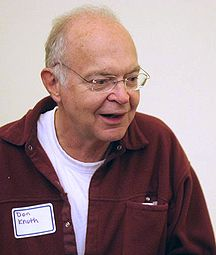
\includegraphics[width=1\linewidth]{knuth1}}
  \end{minipage}
  \hfill
  \begin{minipage}[h]{0.49\linewidth}
    \textbf{Составная \\ подпись 2}
    \center{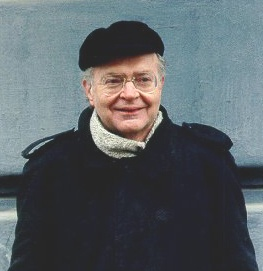
\includegraphics[width=1\linewidth]{knuth2}}
  \end{minipage}
\end{figure}
\end{frame}

\begin{frame}
\frametitle{Таблица}
\begin{tabular}{|l|l|}
\hline
\textbf{Заголовок 1} & \textbf{Заголовок 2} \\
\hline
Сумма & $b+a$ \\
\hline
Разность & $a-b$ \\
\hline
Произведение & $a*b$ \\
\hline
\end{tabular}
\end{frame}

\begin{frame}
\frametitle{Большой многоуровневый список}
\begin{itemize}
  \item \textbf{Пункт 1}
    \begin{itemize}
      \itemi Подпункт 1-1
      \itemi Подпункт 1-2
    \end{itemize}
  \item \textbf{Пункт 2}
    \begin{itemize}
      \itemi Подпункт 2-1
    \end{itemize}
  \item \textbf{Пункт 3}
    \begin{itemize}
      \itemi Подпункт 3-1
      \itemi Подпункт 3-2
    \end{itemize}
  \item \textbf{Пункт 4}
    \begin{itemize}
      \itemi Подпункт 4-1
    \end{itemize}
  \item \textbf{Пункт 5}
    \begin{itemize}
      \itemi Подпункт 5-1
      \itemi Подпункт 5-2
      \itemi Подпункт 5-3
    \end{itemize}
\end{itemize}
\end{frame}

\begin{frame}
\frametitle{Четыре изображения}
\begin{figure}[H]
  \center
    
\includegraphics[width=0.4\linewidth]{latex}
    
\includegraphics[width=0.4\linewidth]{latex}\\
    
\includegraphics[width=0.4\linewidth]{latex}
    
\includegraphics[width=0.4\linewidth]{latex}
\end{figure}
\end{frame}

%%%%%%%%%%%%%%%%%%%%%%%%%%%%%%
\begin{frame}
\frametitle{Перспективы развития проекта}
\begin{itemize}
  \item Перспектива 1
  \item Перспектива 2
  \item Перспектива 3
  \item Перспектива 4
  \item Перспектива 5
\end{itemize}
\end{frame}

\begin{frame}
\frametitle{Результаты работы}
\begin{itemize}
  \item Результат 1
  \item Результат 2
  \item Результат 3
  \item Результат 4
\end{itemize}
\end{frame}

\begin{frame}
\begin{center}
Спасибо за внимание!
\end{center}
\end{frame}

\end{document} 